\chapter{RDF}
\label{chap:rdf}
Das folgende Kapitel basiert auf der Spezifikation des W3C~\cite{w3rdf}.

Die bisherigen Kapitel bieten einen Überblick über die verschiedenen Methoden und Angehensweisen des knowledge engineerings. Die wichtigsten theoretischen Grundlagen wurden in den vorigen Kapiteln erklärt. Im Kapitel~\ref{chap:ontologien}, ``~\nameref{chap:ontologien}'', wurde gezeigt, dass für die Darstellung von Ontologien verschiedene Sprachen entwickelt wurden. 

Wir haben uns für OWL (in der Version 2) entschieden, da es sich um die meistbenutzte Ontologiesprache handelt. OWL wird in der RDF-Syntax verfasst wird, wollen wir letztere erklären.

Das ``Resource Description Framework'' (RDF) ist ein Framework um Informationen aus Ressourcen zu formulieren. Als Ressourcen können Dokumente, Leute, Objekte aber auch abstrakte Inhalte dienen. Im Web können Informationen mit RDF auch verarbeitet werden, anstatt diese nur anzuzeigen. RDF bietet ein gemeinsames Framework um die Informationen zwischen Anwendungen auszutauschen ohne dabei die Bedeutung der Informationen zu verändern.

RDF ist die Grundlage des sematic Web, welches die Flexibilität von RDF vollumfänglich ausnutzt. Alle Daten im semantic Web werden in RDF abgebildet. RDF ermöglicht die Verknüpfung von Daten. Dadurch werden für eine Ressource mehr Informationen zusammen gefügt.\cite{cambSemRDF}

\section{RDF Data Model}
\label{sec:rdf_rdf_dataModel}
In RDF werden Informationen als Aussagen abgebildet. Der Aufbau dieser ist immer gleich und weist die folgende Struktur eines Tripels auf:

\lstset{caption={Tripel-Struktur einer RDF-Aussage},captionpos=b}
\begin{lstlisting}
    <Subjekt> <Prädikat> <Objekt>
\end{lstlisting}

Eine RDF Aussage bildet eine Beziehung zwischen zwei Ressourcen (Entitäten) nämlich Subjekt und Objekt ab. Das Prädikat repräsentiert die Beziehung zwischen den zwei Ressourcen. Die Beziehung wird in RDF als Eigenschaft (Property) abgebildet.

\lstset{caption={Beispiel einer RDF-Aussage},captionpos=b}
\begin{lstlisting}
    <Seilpark> <hatStandort> <Balmberg>
\end{lstlisting}

Eine Entität kann in mehreren Tripeln referenziert werden. Zudem ist es möglich die gleiche Ressource in einer Aussage als Objekt, in einer anderen Aussage als Subjekt zu verwenden. Damit werden Verbindungen zwischen mehreren Tripeln möglich. Dies ist ein wichtiger Aspekt von RDF.\@

Tripel werden in sogenannten RDF-Graphen abgebildet. Diese bestehen aus Knoten und Pfeilen. Subjekte und Objekte werden als Knoten, Prädikate als Pfeile dargestellt. Genaueres dazu findet sich im~\autoref{chap:graph_data}, ``\nameref{chap:graph_data}''.

\begin{figure}[H]
\centering \rotatebox{0}{\scalebox{0.3}[0.3]{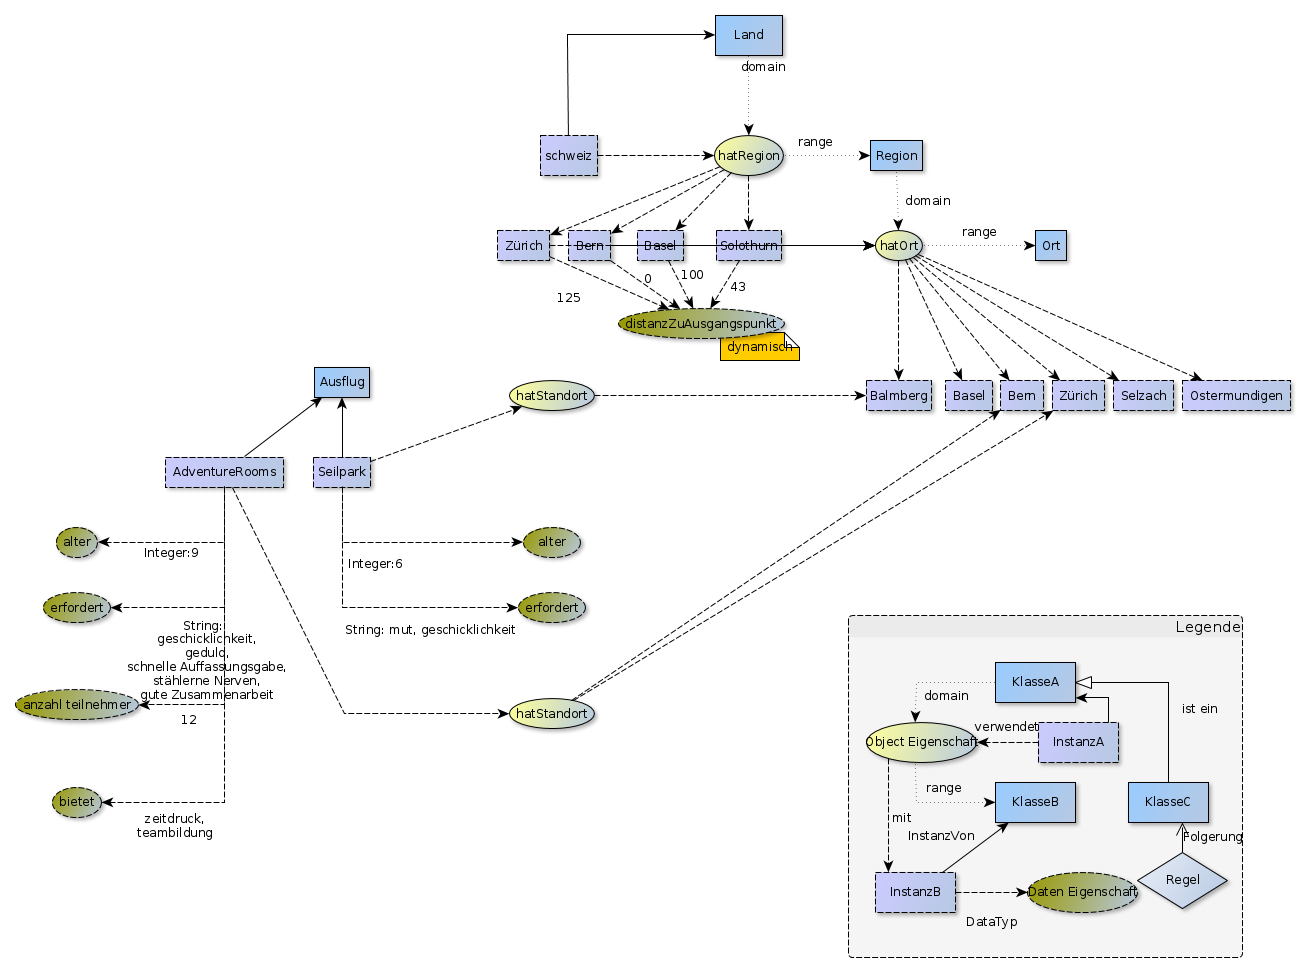
\includegraphics{bilder/rdf_reiseplaner_ontologie.png}}}
\caption{Ausschnitt der Ontologie des Reisplaners\label{fig:rdf_reiseplaner_ontologie}\protect\footnotemark}
\end{figure}
\footnotetext{Eigene Darstellung mittels yEd.}

Man unterscheidet drei Typen von RDF-Daten, welche in Tripeln auftreten: Ressource-Knoten (IRIs), leere Knoten (Blank) und Literale.

\subsection{IRIs (International Resource Identifier)}
\label{sec:rdf_rdf_dataModel_iris}
Wie der Name besagt, stellt ein IRI eine Ressource dar. Dabei handelt es sich um einen globalen Identifier, IRIs können also von verschiedenen Nutzern wiederverwendet werden. Es gibt verschieden Formen von IRIs. Zum Beispiel werden URLs als Web-Adresse verwendet werden. Eine andere Form der IRIs bietet eine Kennung einer Ressource ohne deren Standort oder Zugriff preiszugeben. IRIs können in allen drei Positionen eines Tripels auftreten.

Die genaue Spezifikation von IRIs findet sich unter~\href{http://www.ietf.org/rfc/rfc3987.txt}{RFC 3987}.

\subsection{Literale Knoten}
\label{sec:rdf_rdf_dataModel_literal}
Beim Begriff Literal handelt es sich um ein Synonym für Werte. Literale sind Basiswerte, die nicht IRIs entsprechen. Für die richtige Werteinterpretation wird den Literalen ein Datentyp zugeordnet. Dies können Strings, Datumswerte oder auch Nummern sein. Einem String kann zusätzlich eine Sprache zugewiesen werden.

Literale können in einem Tripel können nur als Objekt verwendet werden.

\subsection{Leere Knoten (blank nodes)}
\label{sec:rdf_rdf_dataModel_blankNodes}
Ein leerer Knoten stellt eine Ressource ohne URI dar. Vorteil:  Diese Knoten benötigen keinen globalen Identifier. Leere Knoten können mit einer einfachen Variablen in der Algebra verglichen werden. Sie bilden ein Objekt ab, wobei der Wert irrelevant ist.

Leere Knoten können in einem Tripel Subjekt oder Objekt darstellen.

\section{Multiple Graphs}
\label{sec:owlRdf_rdf_dataModel_multipleGraphs}
Eine der neuesten Erweiterung von RDF sind multipe Graphen. Diese wurden eingeführt, um Teilmengen einer Tripelsammlung zu definieren. Ursprünglich stammt dieser Mechanismus von der Abfragesprache SPARQL (siehe~\ref{chap:sparql}~\nameref{chap:sparql}). Man unterscheidet zwischen benannten (named) und unbenannten (unnamed) Graphen. Bei unbenannten Graphen enthalten die Tripel jeweils die gesamte URI.\@

\begin{lstlisting}[caption={Beispiel eines unbenannten (unnamed) Graphen}]
	<http://example.org/bob> <is published by> <http://example.org>.
\end{lstlisting}

Bei benannten Graphen wird ein Identifikator (identifier) hinzugefügt, auf welchen referenziert wird.

\begin{lstlisting}[caption={Beispiel eines benannten (named) Graphen}]
Identifier: 
		http://example.org/bob
Graph:
		<Bob> <is a> <person>.
		<Bob> <is a friend of> <Alice>.
\end{lstlisting}

Multipe Graphen eines RDF-Dokumentes stellen eine Datenmenge dar. Sie bestehen standartmässig aus einem unbenannten (unnamed) Graphen und mehreren benannten (named) Graphen. Dabei ist der unbenannte Graph der sog. Basisgraph (default).

\section{RDF Vokabular}
\label{sec:rdf_rdf_voca}
RDF wird typischerweise in Kombination mit einem Vokabular oder anderen Konventionen verwendet, welche semantische Informationen über verwendete Ressourcen bieten.

Um Vokabulare zu definieren, bietet RDF die RDF-Schema-Sprache. Erst diese ermöglicht es semantische Eigenschaften von RDF-Daten zu definieren. Damit kann beispielsweise festgelegt werden, welche Ressourcen an welcher Position eines Tripels verwendet werden sollen.

RDF verwendet den Klassen-Bezeichner (class) um Kategorien zu definieren, welche die Klassifizierung von Ressourcen erlauben. Die Beziehung zwischen einer Instanz und ihrer Klasse wird durch den Typen-Bezeichern (type) ausgedrückt. 

Mit der RDF-Schema-Sprache können Hierarchien im Bereich der Klassen und Sub-Klassen sowie der Eigenschaften und Untereigenschaften gebildet werden. Auf Subjekten bzw. Objekten können Typeneinschränkungen mittels dem Domänen- (domain) bzw.\ dem Bereichs-Bezeichner (range) vorgenommen werden.~\footnote{http://www.w3.org/TR/2014/NOTE-rdf11-primer-20140624/\#section-rdfa~\cite{w3rdf}}

\section{RDF Formen}
\label{sec:rdf_rdf_formen}
RDF kann in verschiedenen Formen niedergeschrieben werden. Sie alle führen zu den exakt selben Tripeln, sind also logisch äquivalent. Die Einsatzgebiete sind jedoch unterschiedlich.
Formen von RDF sind: Turtle-Schreibweise (N-Triples, Turtle, TriG und N-Quads), JSON-LD, RDFa und RDF/XML.\@

Da wir letztere Schreibweise in unserem Beispiel verwendet haben, werden wir sie genauer vorgestellen.

\subsection{RDF/XML}
\label{sec:rdf_rdf_formen_xmlRdf}
Bei RDF/XML handelt es sich um eine Schreibweise von RDF, welche die XML-Syntax verwendet. Bei der Entwicklung von RDF in den 1990er Jahren, war RDF/XML die einzig existierende Schreibweise.

In RDF/XML werden Tripel in dem XML-Element, \textit{rdf:RDF}, spezifizert. Das XML-Element \textit{rdf:description} definiert eine Menge von Tripeln, welche als Subjekt den IRI ihres \textit{about}-Attributes haben.

Ein Description-Element kann Unterelemente beinhalten. Der Name des Unterelementes ist ein IRI, welcher in der RDF-Eigenschaft \textit{rdf:type} abgebildet ist. Dabei repräsentiert jedes Unterelement ein Tripel.

Handelt es sich bei dem Objekt eines Tripels auch um einen IRI, hat das Unterelement keinen Inhalt und der Objekt-IRI-Knoten wird durch das \textit{rdf:resource}-Attribut beschrieben.

Ist das Objekt eines Tripels ein Literal, wird der Inhalt der RDF-Eigenschaft zum Literalwert.\\
Der Datentyp der RDF-Eigenschaft wird durch als Attribut angegeben. Bei Fehlen von Datentyp und Sprache wird angenommen, dass der Literal vom Datentyp ``String'' ist.

\begin{lstlisting}[caption={Beispiel RDF Elemente\protect\footnotemark}]
<!DOCTYPE rdf:RDF [
    <!ENTITY owl "http://www.w3.org/2002/07/owl#" >
    <!ENTITY swrl "http://www.w3.org/2003/11/swrl#" >
    <!ENTITY swrlb "http://www.w3.org/2003/11/swrlb#" >
    <!ENTITY xsd "http://www.w3.org/2001/XMLSchema#" >
    <!ENTITY rdfs "http://www.w3.org/2000/01/rdf-schema#" >
    <!ENTITY rdf "http://www.w3.org/1999/02/22-rdf-syntax-ns#" >
]>


<rdf:RDF xmlns="http://www.semanticweb.org/mira/ontologies/2014/9/FamilyOnto#"
     xml:base="http://www.semanticweb.org/mira/ontologies/2014/9/FamilyOnto"
     xmlns:rdfs="http://www.w3.org/2000/01/rdf-schema#"
     xmlns:swrl="http://www.w3.org/2003/11/swrl#"
     xmlns:owl="http://www.w3.org/2002/07/owl#"
     xmlns:xsd="http://www.w3.org/2001/XMLSchema#"
     xmlns:swrlb="http://www.w3.org/2003/11/swrlb#"
     xmlns:rdf="http://www.w3.org/1999/02/22-rdf-syntax-ns#">
    <owl:Ontology rdf:about="http://www.semanticweb.org/mira/ontologies/2014/9/FamilyOnto"/>
    <rdf:Description>
        <rdf:type rdf:resource="&swrl;IndividualPropertyAtom"/>
        <swrl:propertyPredicate rdf:resource="http://www.semanticweb.org/mira/ontologies/2014/9/FamilyOnto#isAncestor"/>
        <swrl:argument1 rdf:resource="urn:swrl#a"/>
        <swrl:argument2 rdf:resource="urn:swrl#x"/>
    </rdf:Description>
</rdf:RD>
\end{lstlisting}
\footnotetext{Eigenes Beispiel}
